% Project report for Visual Analytics (602AA) - VAST Challenge 2025, Mini-Challenge 3 (English version)
% Build: tectonic report_en.tex (or pdfLaTeX). Figures are in ../docs/screenshots/ and ../docs/mockups/.
\documentclass[11pt,a4paper]{article}

\usepackage[utf8]{inputenc}
\usepackage[T1]{fontenc}
\usepackage[english]{babel}
\usepackage[a4paper,margin=2.3cm]{geometry}
\usepackage{lmodern}
\usepackage{microtype}
\usepackage{booktabs}
\usepackage{tabularx}
\usepackage{graphicx}
\graphicspath{{../docs/screenshots/}{../docs/mockups/}{fig/}}
\usepackage{enumitem}
\usepackage{caption}
\usepackage{float}
\usepackage[hidelinks]{hyperref}

\setlist{leftmargin=1.4em,itemsep=2pt,topsep=3pt}
\captionsetup{font=small,labelfont=bf}
\renewcommand{\arraystretch}{1.15}

\begin{document}

\begin{titlepage}
\centering
\vspace*{3cm}
{\large Visual Analytics\par}
\vspace{0.4cm}
{\normalsize University of Pisa\par}
\vspace{2.5cm}
{\huge\bfseries Project Report\par}
\vspace{0.8cm}
{\large Analysing the radio communications of Oceanus\par}
\vspace{0.2cm}
{\large VAST Challenge 2025, Mini-Challenge 3\par}
\vfill
{\normalsize Student: Giuseppe Vincenzo Dylan Toscano (599752)\par}
\vspace{0.4cm}
{\normalsize Academic Year 2025--2026\par}
\vspace*{2.5cm}
\end{titlepage}

\tableofcontents
\newpage

%---------------------------------------------------------------------
\section{Introduction}
%---------------------------------------------------------------------
This project proposes a solution to Mini-Challenge 3 of the VAST Challenge 2025, set on the island of Oceanus.
The journalist Clepper Jensen recorded the radio communications intercepted on the island for two weeks
(1--14 October 2040) and, with the help of an intern, turned them into a knowledge graph of the events and of the
relationships between the people involved. Most messages are about Nemo Reef, a protected marine area whose closure
is announced on 10 October, while an event of the singer Sailor Shift is being prepared on the island.

The challenge asks four questions:
\begin{enumerate}
  \item what the daily patterns of the communications are, how they change over the two weeks and which entities
        have influence over a chosen entity;
  \item which groups of people and vessels can be identified and which topics each group talks about;
  \item who uses pseudonyms (Boss, The Middleman, Mrs.\ Money and others) and who is behind them;
  \item whether Nadia Conti, formerly entangled in an illegal fishing scheme, is still involved in illicit activity.
\end{enumerate}

The goal is an interface that lets the journalist answer these questions without help. The journalist knows the
context well but is not a graph expert. For this reason I avoided drawing the whole graph as a tangle of nodes and
edges, and every graphical element leads to the text of the messages it comes from, which for a journalist is the
actual evidence.

All the charts are built with D3.js, including the original view required by the course (Section~\ref{sec:orig}).
Pages and filters are handled with Vue.js and styling with Tailwind CSS; data preparation is done in Python (pandas and
networkx). The repository contains the data preparation (\texttt{scripts/}), the application (\texttt{app/}) and the
exploration notebook with the mockups (\texttt{analysis/}, \texttt{docs/}); start-up instructions are in
\texttt{README.md}. The
challenge data are not included and must be downloaded from the VAST Challenge website. The interface is in
Italian: in this report its titles and labels are quoted in English translation.

%---------------------------------------------------------------------
\section{Data understanding and data preparation}
%---------------------------------------------------------------------
\subsection{Structure of the graph}
\texttt{MC3\_graph.json} is a directed graph with 1159 nodes and 3226 edges. Nodes are of three kinds: 72 entities
(people, vessels, organisations, locations, groups), 802 events, of which 584 are radio communications, and 285
relationship nodes. Relationships are reified: a relationship between two entities (for example \emph{Colleagues}
or \emph{Operates}) is a node linked to both entities, and \texttt{evidence\_for} edges link the messages to the
relationships they support. The \texttt{sent} and \texttt{received} edges give the sender and the recipient of each
message according to the radio metadata.

For the analysis the graph was turned into tables: one for the messages (sender, recipient, date, text), one for the
relationships between pairs of entities and one for the evidence linking messages and relationships. After cleaning,
581 messages remain (3 exact duplicates were removed), exchanged by 40 actors (17 people, 14 vessels,
5 organisations and 4 locations), and 192 relationships between these actors, each with the list of messages that
support it.

The messages cover all 14 days, with 34--49 messages per day, and they are sent only between 8:00 and 15:00, with a
peak at 10:00 (146 messages). This is also the time band shown in the calendar of the first page.

\subsection{Recorded sender and real sender}\label{sec:senders}
Almost every message opens with a call formula such as ``Davis, Mako here'', which tells that Mako is writing to
Davis. These formulas were recognised in 569 messages out of 584 and compared with the sender and the recipient
recorded by the radio. The comparison gave these results:
\begin{itemize}
  \item in 80 messages the graph has a sender or a recipient different from the text: in 76 the sender is wrong and
        in 4 only the recipient;
  \item of the 76 messages with a wrong sender, 43 have sender and recipient swapped and 31 appear to be sent to
        oneself (for example Davis $\rightarrow$ Davis with the text ``Davis, Mako here''). In all these 74 cases the
        radio recorded the recipient in place of the sender;
  \item 2 messages remain whose difference cannot be explained this way; they are discussed in
        Section~\ref{sec:q3}.
\end{itemize}
At first I read the signatures that differ from the sender as possible pseudonyms. The unusual number of messages
sent to oneself made me check the texts again, and it turned out that in most cases the radio had recorded the wrong person as the sender. This step
matters for the third question, because otherwise we would have looked for pseudonyms that do not exist. Every
message keeps both the corrected values and the original radio values, and the interface can switch back to the
original data.

\subsection{Derived data}
Some additional data were computed on top of the tables:
\begin{itemize}
  \item \textbf{Groups}: computed with the Louvain algorithm, which puts in the same group the actors that exchange
        many messages with each other and few with the rest. I named each group after a well-known member or after
        what its members do: Nemo Reef
        Operation (15 actors, including Nadia Conti, Davis and the vessels Mako and Remora), Control and institutions
        (15 actors, including the Oceanus City Council, the harbours, the Green Guardians and the patrol vessels),
        Aliases (the 8 pseudonyms) and Investigators (Clepper Jensen and Miranda Jordan).
  \item \textbf{Topics}: ten topics found with keywords, for example \emph{permits} (``permit'', ``authoriz'',
        ``clearance''), \emph{money / payments}, \emph{equipment / works} and \emph{secrecy}. A message can have more
        than one topic. The method is approximate, but the rules are easy to check and the messages found for each
        topic can be read.
  \item \textbf{Cited times}: the times written in the text of the messages (for example ``meet at 0500'' or
        ``7PM''), 169 in total.
  \item \textbf{Suspicious actions}: reading the messages of Nadia Conti and Boss I marked by hand 24 suspicious
        actions (18 of Nadia and 6 of Boss), divided into six types, plus one piece of counter-evidence. Each action is linked to the message it comes from, so it can be checked.
\end{itemize}

%---------------------------------------------------------------------
\section{Design and functioning of the interface}
%---------------------------------------------------------------------
\subsection{State of the art}
The most common way to show a knowledge graph is to draw all of it as nodes and edges, with positions computed by a
force-directed algorithm. With 40 actors and a few hundred links the result is a tangle that is hard to read,
especially for someone who is not a graph expert. I therefore preferred views that aggregate the data and put time on
an axis (calendar, timeline), a graph split into areas, one per group, and, to compare two versions of the same data, a
ribbon chart linking two lists of names. The typical problem of this challenge, senders recorded in the wrong way, is
not solved just by showing it: the analyst also needs a way to decide which version to use and to
see what changes in the rest of the analysis, and this is where the original view comes from
(Section~\ref{sec:orig}).

\subsection{Model and communication pattern}
The interface has one page for each question of the challenge, and the question is written at the top of the page.
Every page reads in the same order: first the charts with the overall picture, then the filters to narrow it down,
finally the text of the single messages when an element is clicked. The user can explore freely, but there are a few
starting points already set: for example the
first and the fourth page open with Nadia Conti already selected.

A common bar at the top contains the navigation between pages, the field to choose an actor and the filters for
group, period (14 days, first week, second week) and topic, with the number of selected messages. The actor and the
filters apply to all pages, and clicking an actor in one view selects it in the others too. On the right there is
always the message panel: clicking an element of a chart (a tick, a bar, a cell, an edge or a ribbon) shows in the
panel the text of the messages behind that element.

\subsection{Design choices: colours, shapes and interactions}
\paragraph{Colours.} Colour identifies the group of the actor and is the same in every view: orange for the Nemo Reef
Operation, green for Control and institutions, pink for the Aliases and blue for the Investigators. They are colours of
the Okabe-Ito palette, chosen because it stays distinguishable for colour-blind people. Quantities, as in
the topic table, use the reversed magma scale, from light to dark; viridis was discarded because its green is too
close to the one of Control and institutions. The two weeks use the same purple at two lightness levels, because they
are ordered data. Grey is used only for backgrounds and context, never for a quantity. Coloured text was darkened to
reach a contrast of at least 4.5:1 with the background.

\paragraph{Shapes and encodings.} The type of actor is shown by the shape of the symbol: circle for people, triangle
for vessels, square for organisations, diamond for locations. Quantities to be compared are encoded by position on a
common scale or by the length of bars starting from zero, because these are read most accurately (ranking of Cleveland
and McGill). Area is used only for the size of the nodes in the graph, where it is enough to see who is more active. Less
certain elements are drawn lighter or hollow: for example relationships supported by a single message, or actions
reported by others.

\paragraph{Titles.} The title of each chart describes what the chart shows, for example ``The busiest day is
11 October (49 messages): Nemo Reef closure''. Titles are computed from the data displayed, so they change with the
filters and with the chosen actor. How to read each chart is explained under the \textsf{i} symbol next to the title.

\paragraph{Interactions.} Every chart has a tooltip on mouse hover. Clicking an element opens the corresponding
messages in the panel on the right; clicking an actor selects it in all pages and highlights it in the views. The graph
of the second page can be zoomed with the mouse wheel, and in the calendar a day can be clicked to enlarge it.

\subsection{Structure of the interface}
\subsubsection{Q1: rhythms and influence}
\begin{figure}[!htbp]\centering
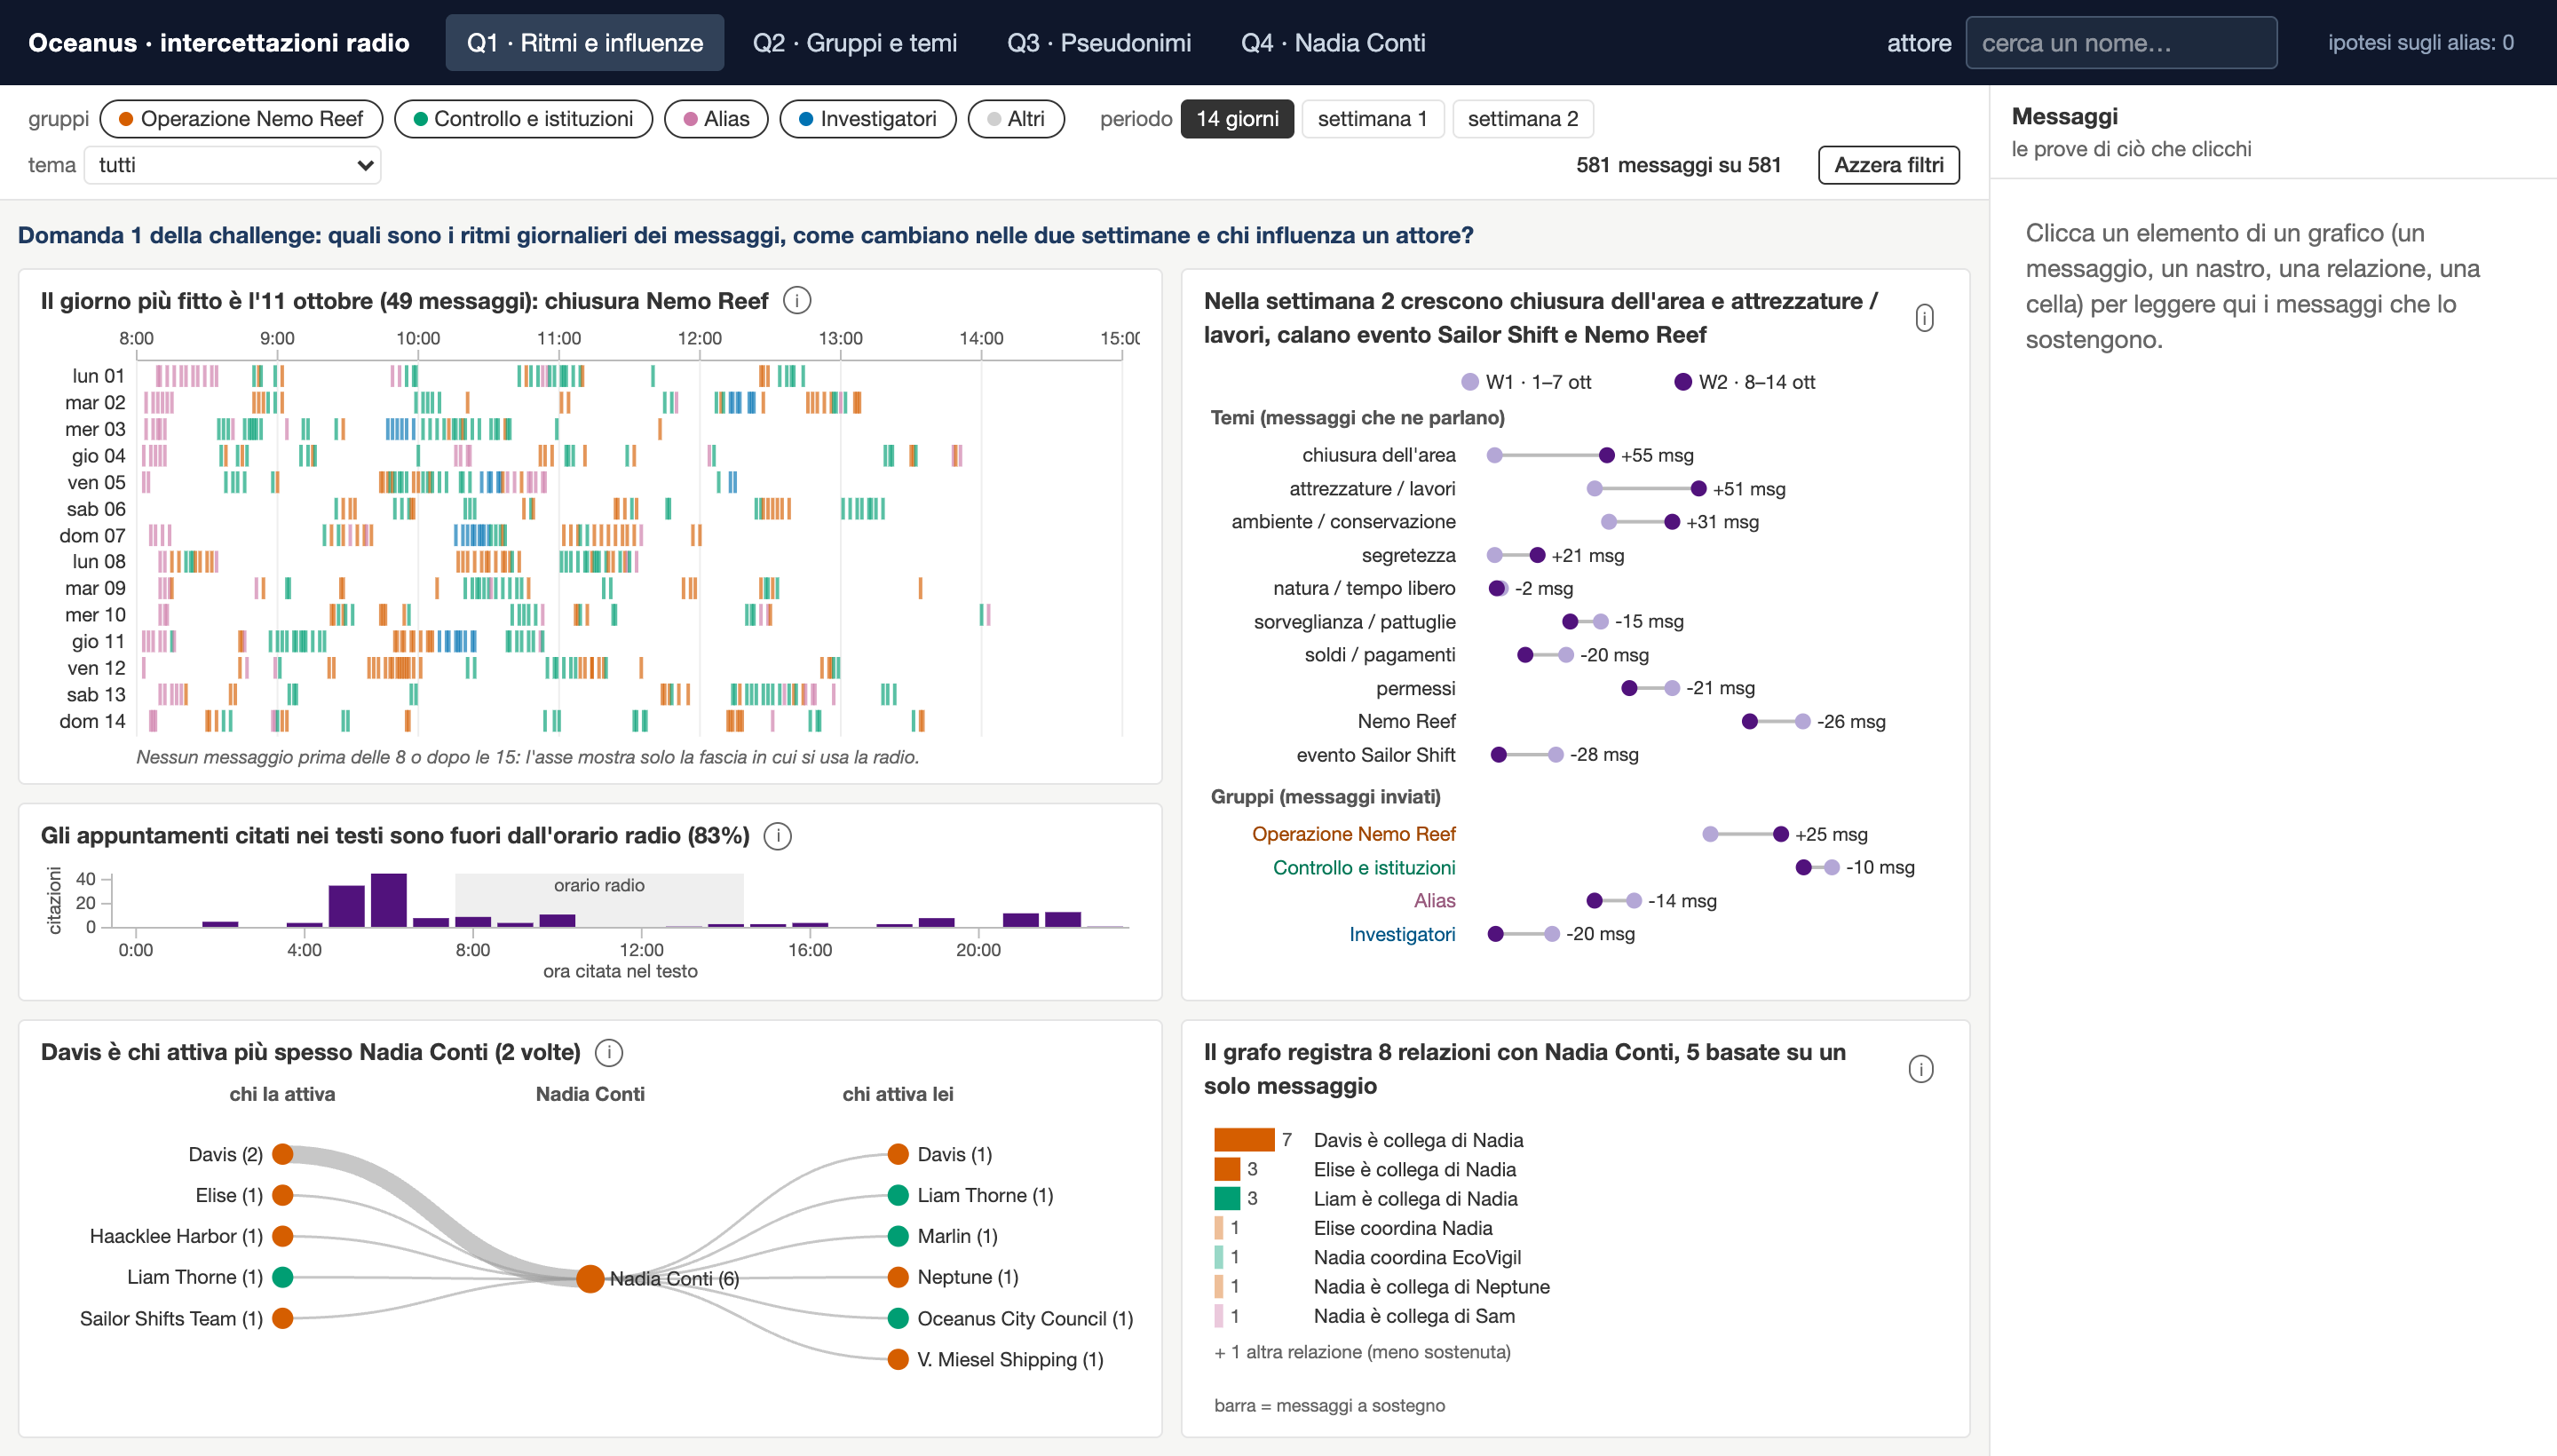
\includegraphics[width=\linewidth]{01_q1_ritmi.png}
\caption{First page: calendar of the messages and times cited in the texts (left), comparison between the two weeks
(right), who activates the chosen actor and its relationships in the graph (bottom).}\label{fig:p1}
\end{figure}
The main widget is a calendar with one row per day and the time of day on the horizontal axis (from 8:00 to 15:00).
Each message is a tick coloured by the group of its sender. I had considered a heatmap with one-hour cells, but the
aggregation hid the sequences of messages a few minutes apart, which are frequent in this dataset. Under the calendar
a bar chart shows the times cited in the texts over the 24 hours, with the band in which the radio is used shaded in
grey.

On the right, a dumbbell chart compares the first and the second week for each topic and each group on the same scale;
rows are sorted by the largest increase and the difference is written next to them (for example ``+55 msg''). At the
bottom there are two widgets about the chosen actor. The first shows on the left who writes to the actor shortly
before the actor writes to someone else (within 15 minutes) and on the right whom the actor writes to right after,
with the width proportional to the number of times. It measures precedence in time and does not prove a chain of
command. The second lists the relationships that the graph records for the actor, written as sentences (``Davis
is a colleague of Nadia'') together with the number of messages that support them.

\subsubsection{Q2: groups and topics}
\begin{figure}[!htbp]\centering
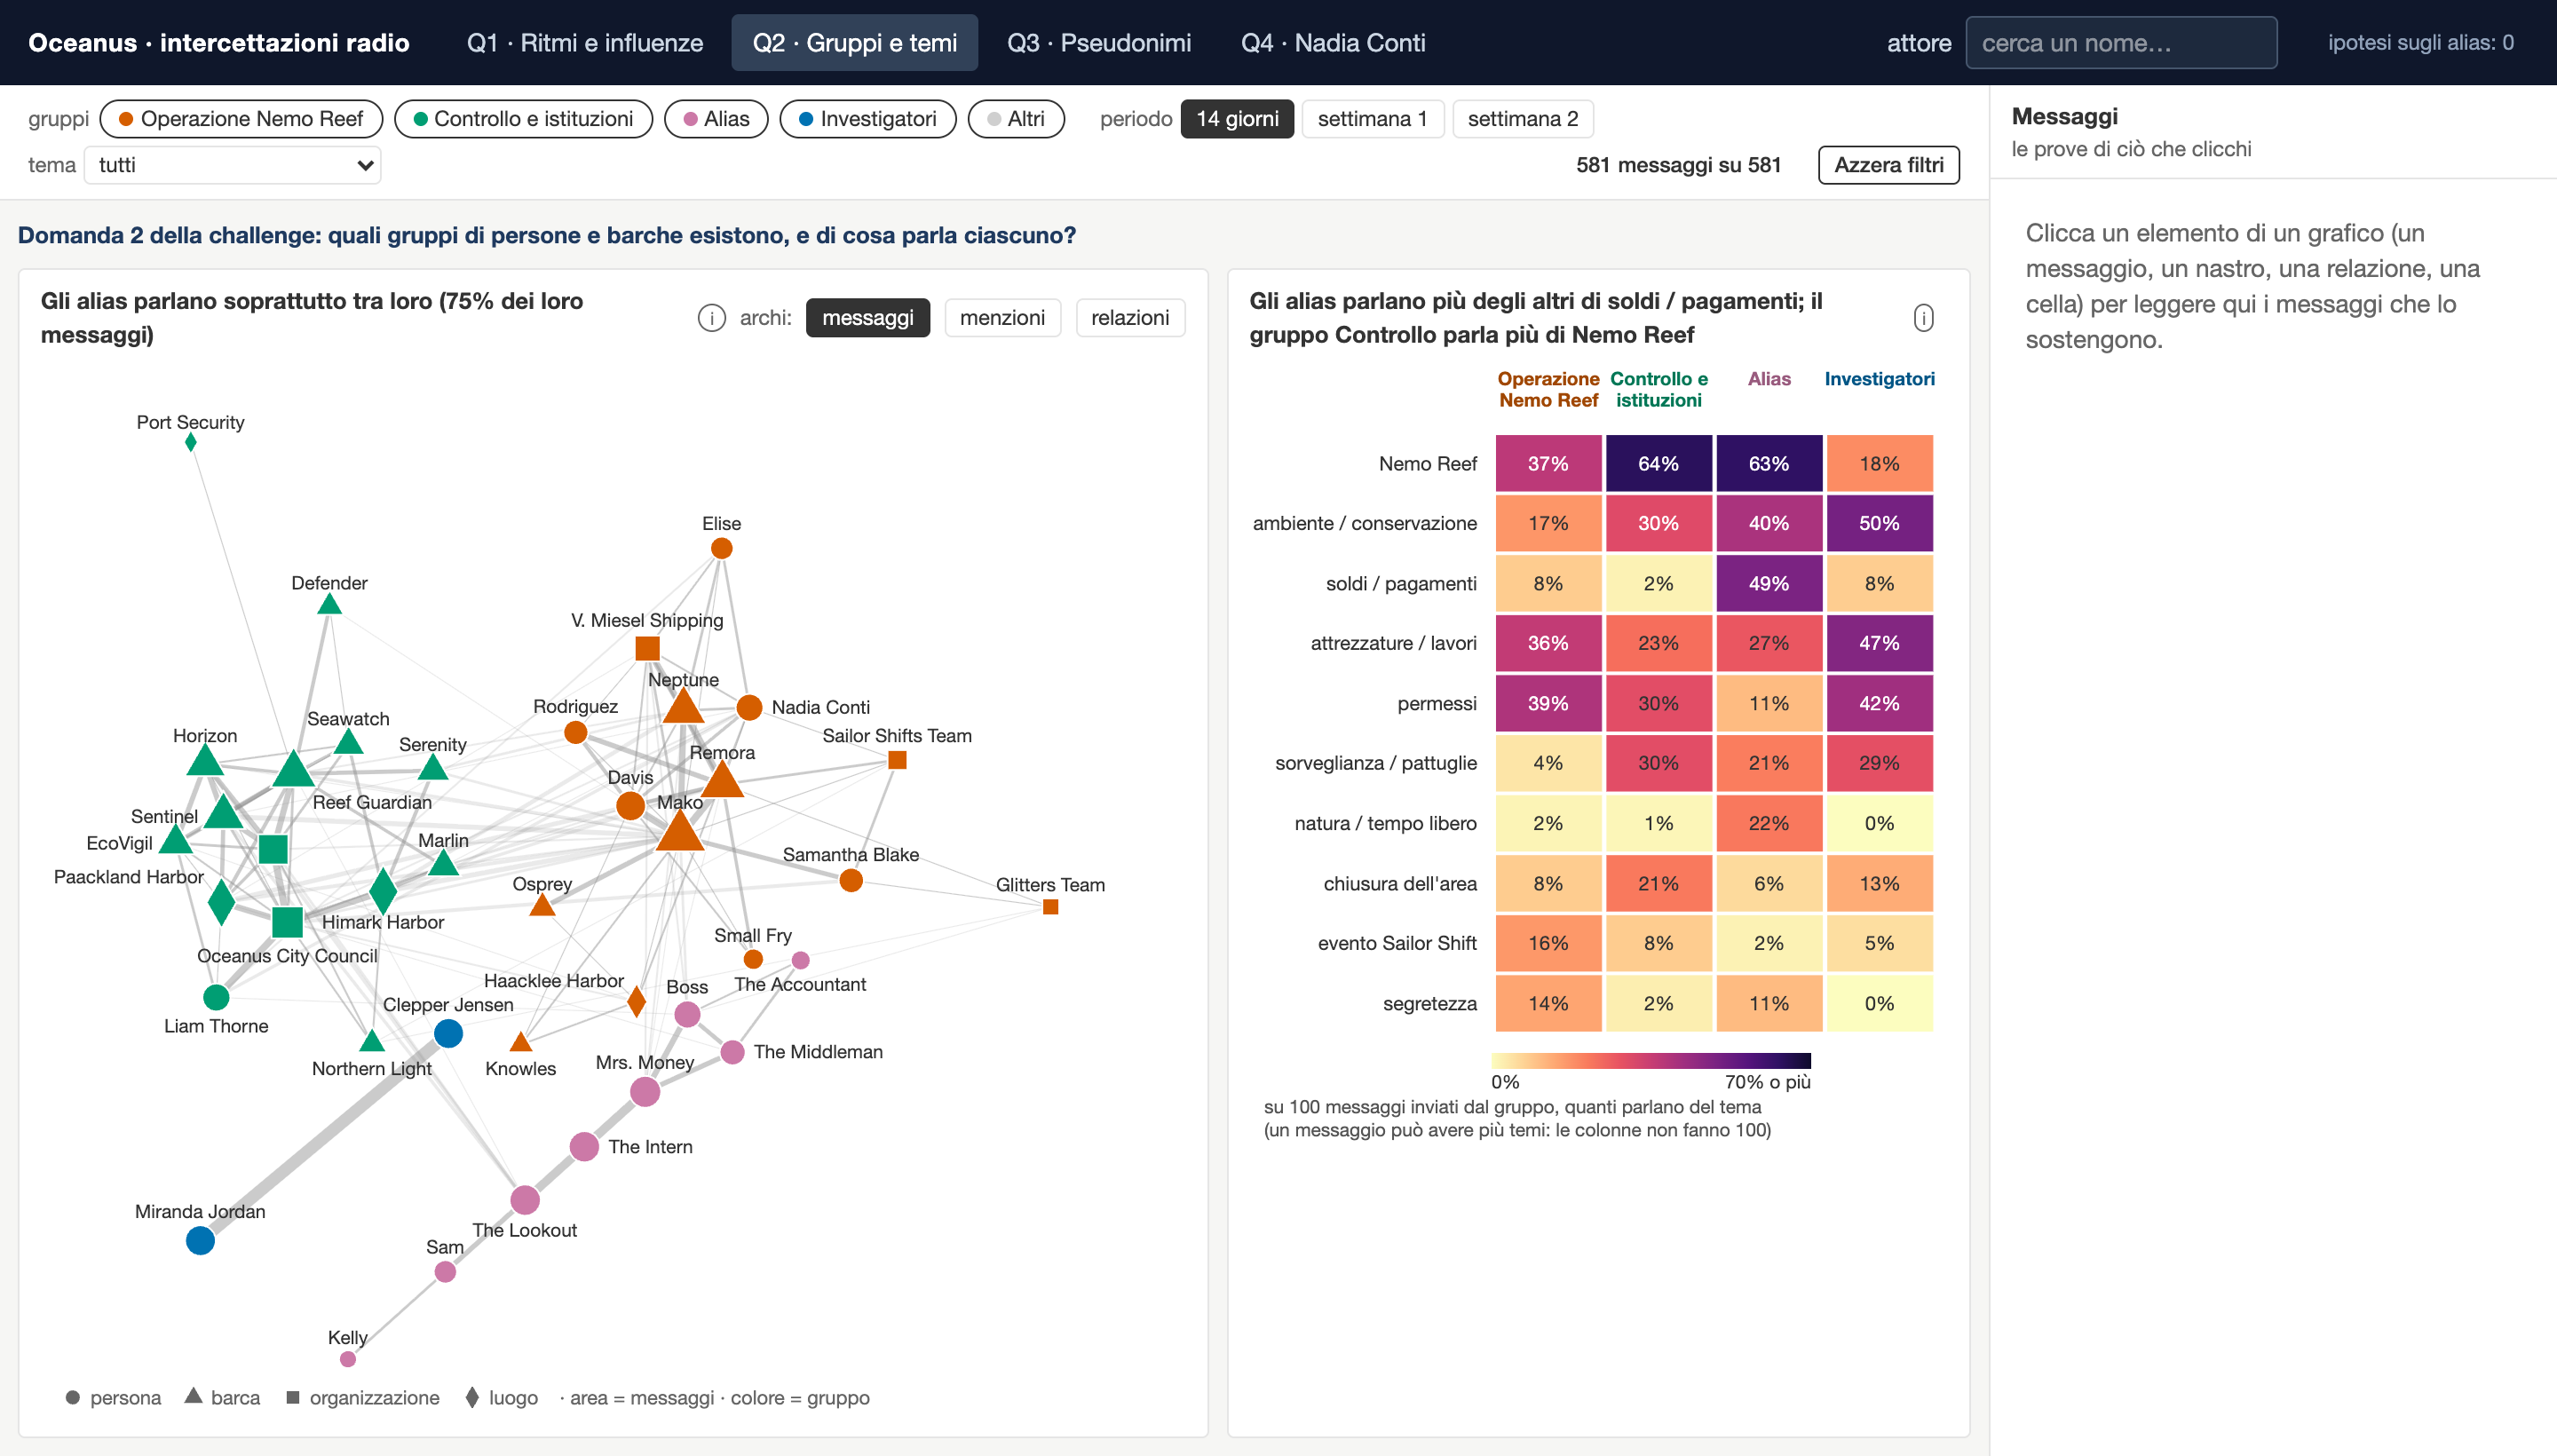
\includegraphics[width=\linewidth]{07_q2_gruppi_messaggi.png}
\caption{Second page: the graph of the actors with one area per group, and the table of topics per group.}\label{fig:p2}
\end{figure}
The graph shows the 40 actors split into four areas, one per group, and the nodes always stay in the same place. A
button chooses which links to draw on the same nodes: the
messages exchanged, the mentions in the text and the relationships of the graph. Links between different groups are
lighter than links inside a group, so the blocks are seen first; labels are placed so that they do not overlap. The
table next to it has topics on the rows and groups on the columns; each cell tells how many messages out of 100 sent
by the group talk about that topic.

\subsubsection{Q3: pseudonyms}
\begin{figure}[!htbp]\centering
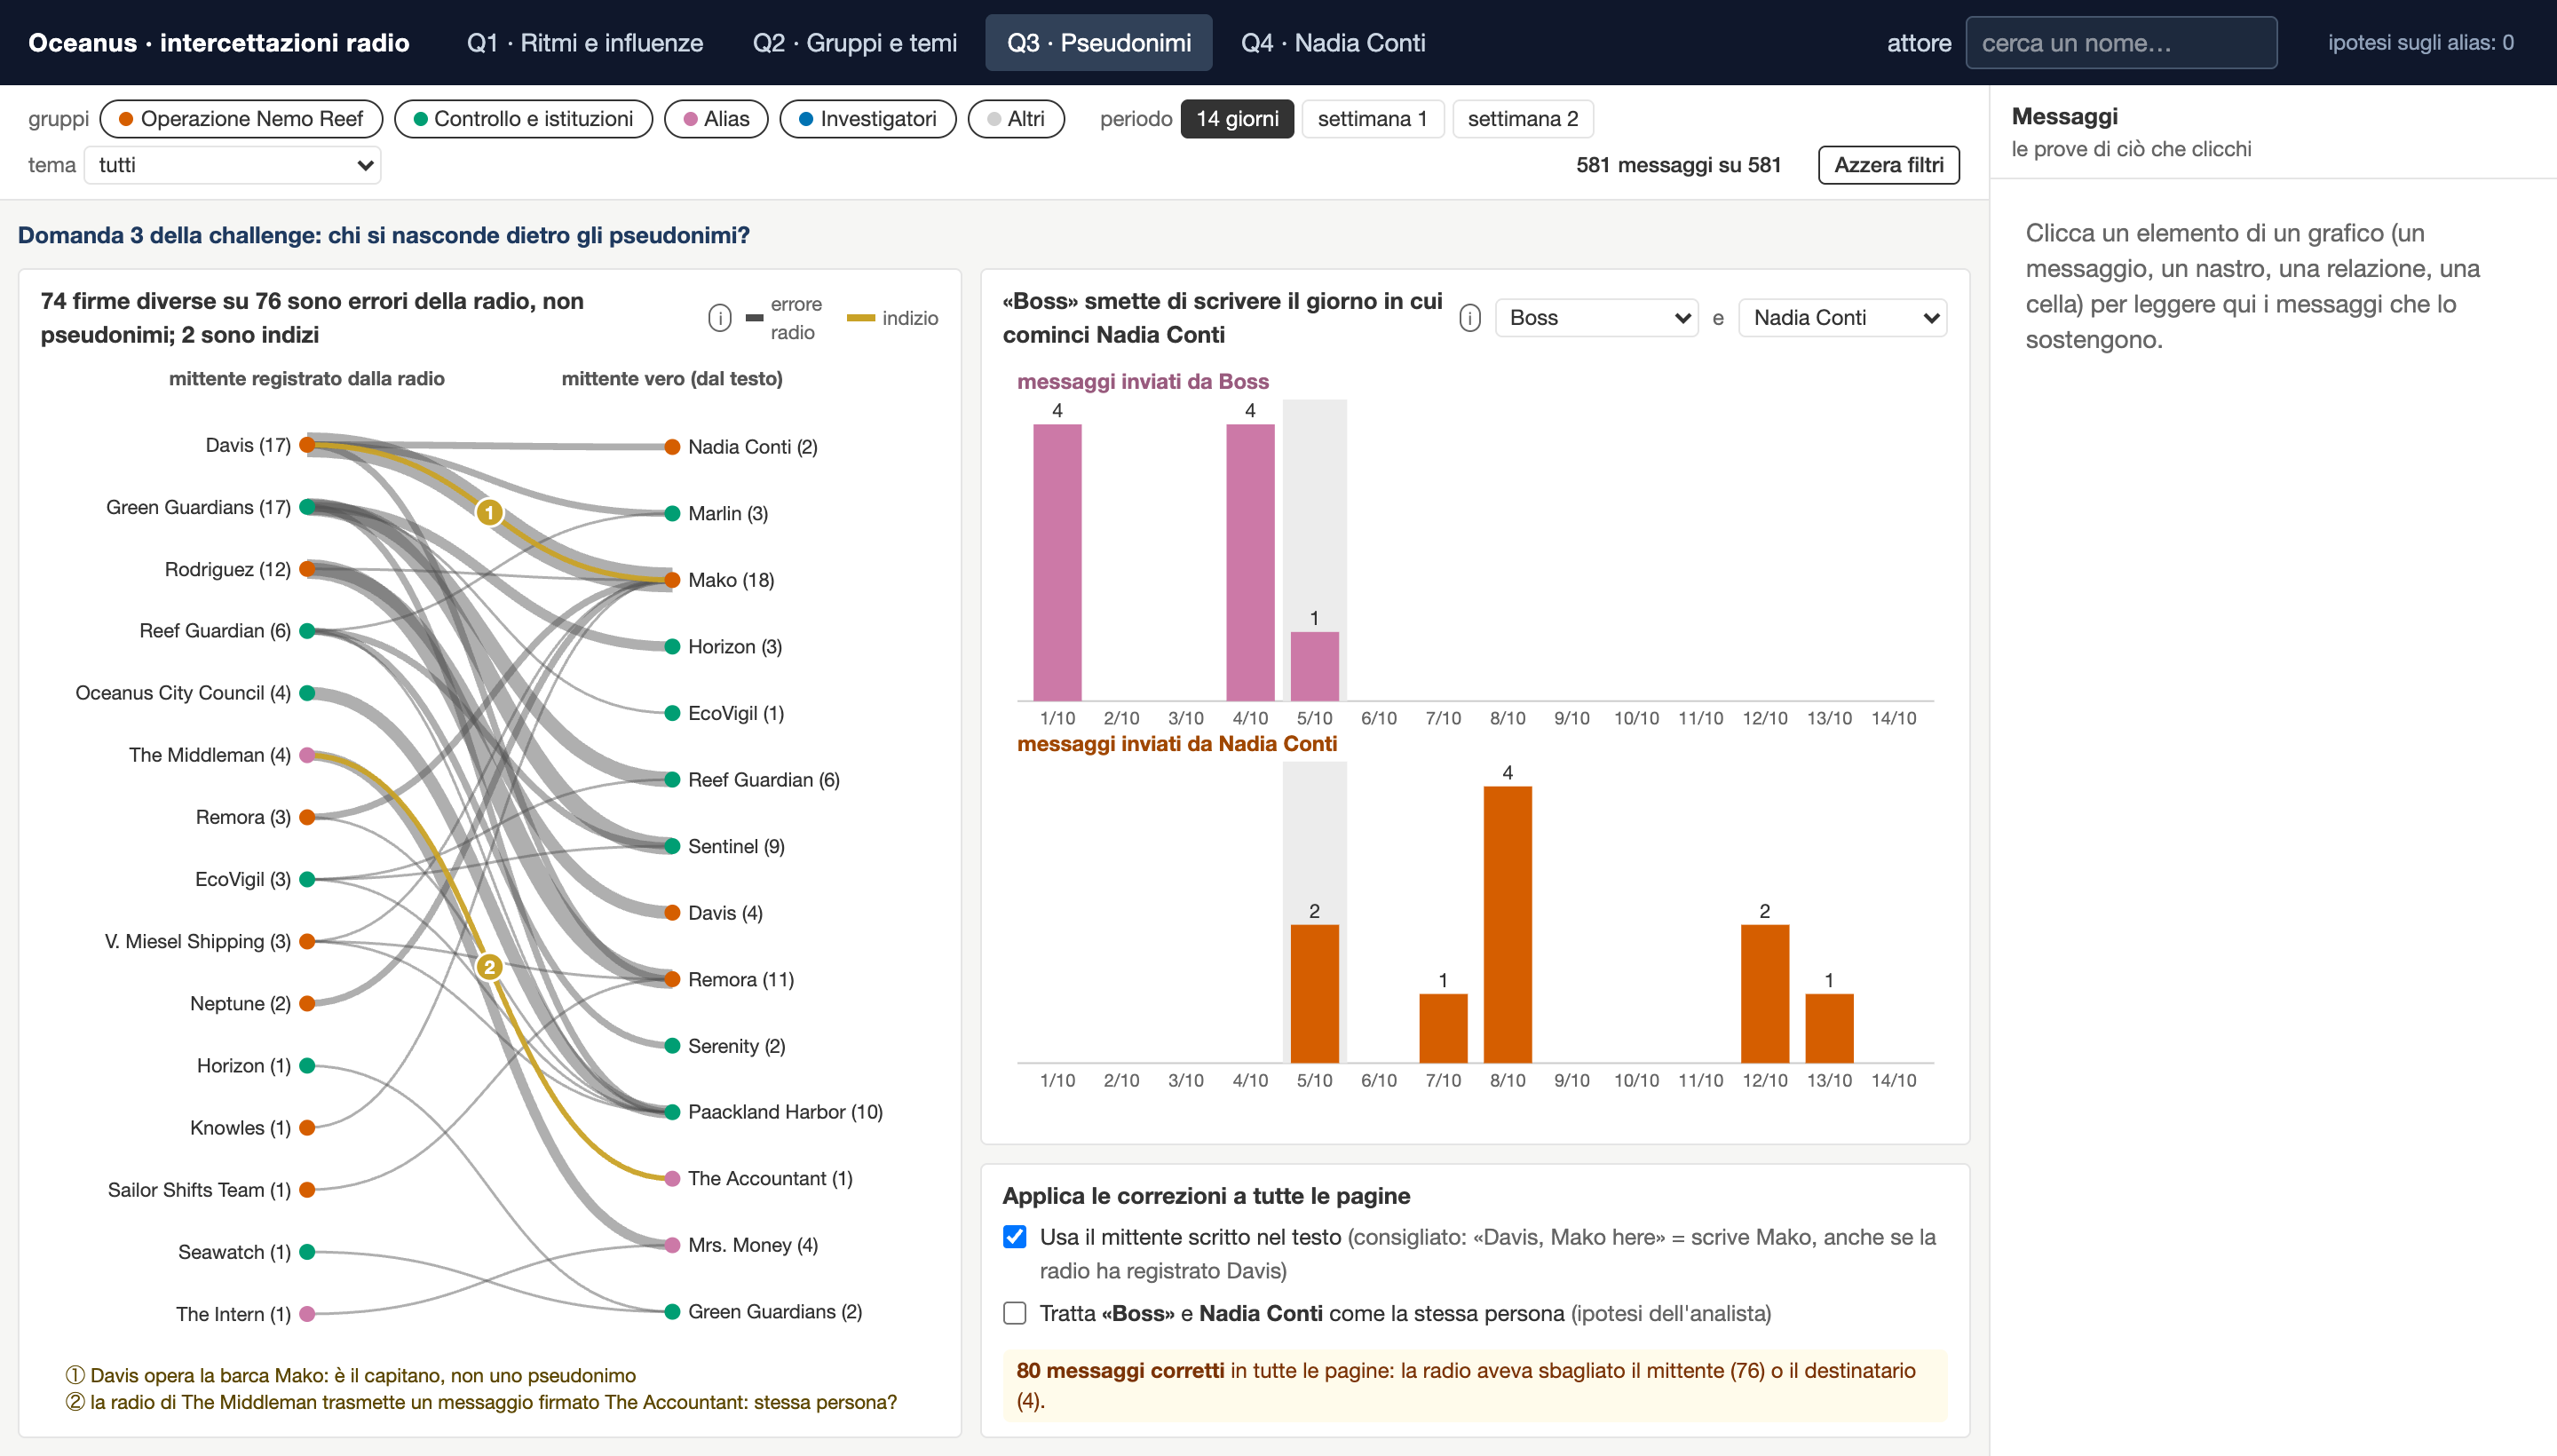
\includegraphics[width=\linewidth]{04_q3_mittenti_veri.png}
\caption{Third page: on the left the original view (recorded sender and real sender), on the right the messages sent
each day by an alias and by a candidate, and the corrections panel.}\label{fig:p3}
\end{figure}
The page has three parts. On the left is the original view (Section~\ref{sec:orig}). At the top right two menus choose
an alias and a candidate, for example Boss and Nadia Conti: the chart shows how many messages each of them sends every
day, the alias on top and the candidate below on the same scale, and the days on which both write are shaded in grey.
At the bottom right there are two checkboxes that apply to the whole application: the first uses the sender written in
the text instead of the one recorded by the radio, the second treats the chosen alias and candidate as the same person.

Before reaching this version I had tried a similarity matrix between aliases and candidates, based on shared contacts
and days: for Boss all candidates scored between 13\% and 14\%, so it did not help to tell them apart.

\subsubsection{Q4: Nadia Conti}
\begin{figure}[!htbp]\centering
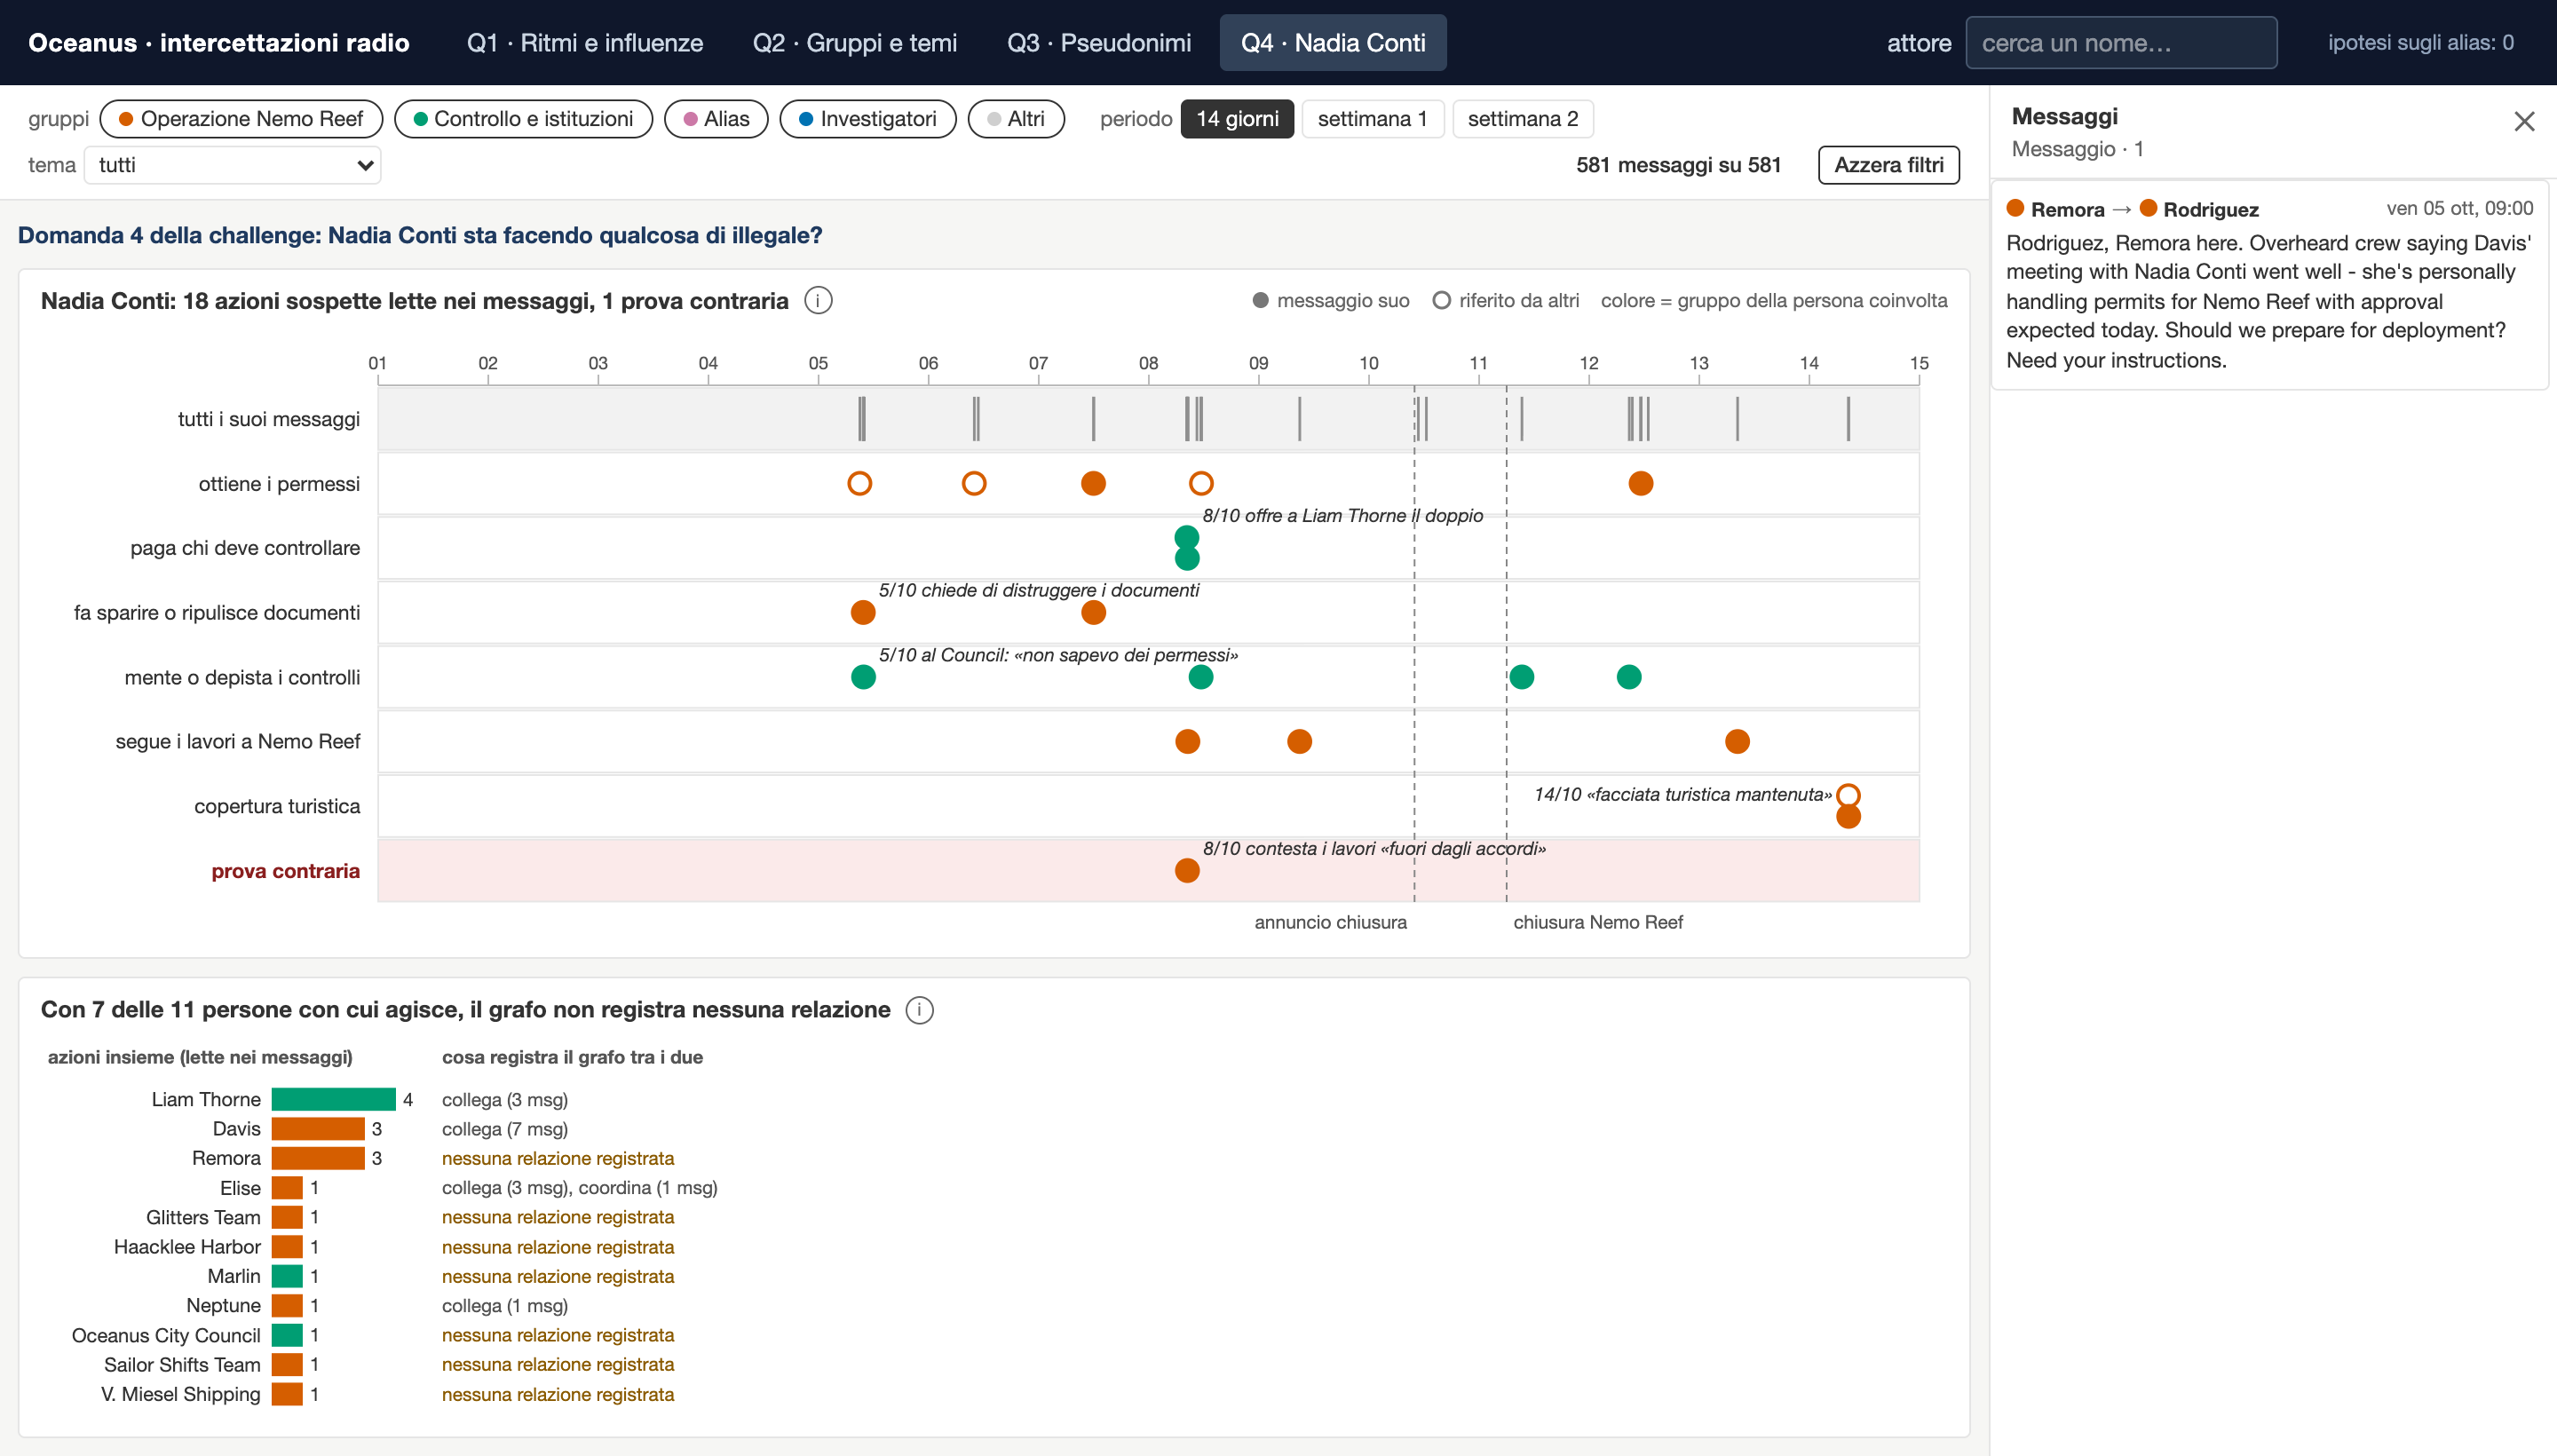
\includegraphics[width=\linewidth]{06_q4_azioni_nadia.png}
\caption{Fourth page: the actions of Nadia Conti over time and the people she acts with; on the right the selected
message.}\label{fig:p4}
\end{figure}
The timeline has one row for each type of action (obtains permits, pays those who should control, makes documents
disappear, lies to or misleads the controls, follows the works at Nemo Reef, tourist cover) and at the bottom a row
for the counter-evidence. A filled circle is a message written or received by her, a hollow one an action reported by
others, a dashed one an action attributed through a hypothesis of the third page; colour is the group of the person
involved. At the top are all the messages in which she appears, and the dashed lines mark the announcement of the
closure and the closure of Nemo Reef. The chart below lists the people she acts with and, for each of them, the
relationship the graph records between the two.

\subsection{The original view}\label{sec:orig}
The original view is the ribbon chart of the third page. On the left there is the sender recorded by the radio, on the
right the one written in the text, and each ribbon links a pair with a width proportional to the number of messages.
It was built in D3 and has four features.
\begin{enumerate}
  \item Every discrepancy is classified automatically (sender and recipient swapped, message to oneself, other). The
        ribbons of radio errors are grey; the cases that cannot be explained as an error get a separate yellow ribbon,
        even when they link the same names as a grey ribbon.
  \item The two yellow ribbons carry a number, and their explanation is written under the chart, derived from the
        relationships of the graph: if the recorded sender operates the vessel that signs the message, the view says so.
  \item The order of the names on the right is computed to reduce crossings: each name is placed at the mean position
        of its senders on the left (barycentre method) and then neighbouring names are swapped as long as crossings
        decrease. Weighting each crossing by the width of the two ribbons, crossings go from 1031 (names sorted by
        number of messages) to 544. The ribbon under the mouse is brought to the front.
  \item The choices made here apply to the whole application. If the correction is turned off, every page goes back
        to the original radio data (80 messages change); if a hypothesis about an alias is turned on, the alias is
        merged with the person in every view: the Boss node disappears from the graph of the second page, the chart of
        who activates whom on the first page is recomputed and in the fourth page the actions of Boss appear, dashed
        (Fig.~\ref{fig:hypothesis}).
\end{enumerate}
The shape of the chart is that of an ordinary bipartite diagram. What is new is its use to audit the graph: colour
shows the type of error, the clues are explained with a second source, and the analyst can decide which corrections
to apply and immediately see the before and after in the other pages.

\begin{figure}[!htbp]\centering
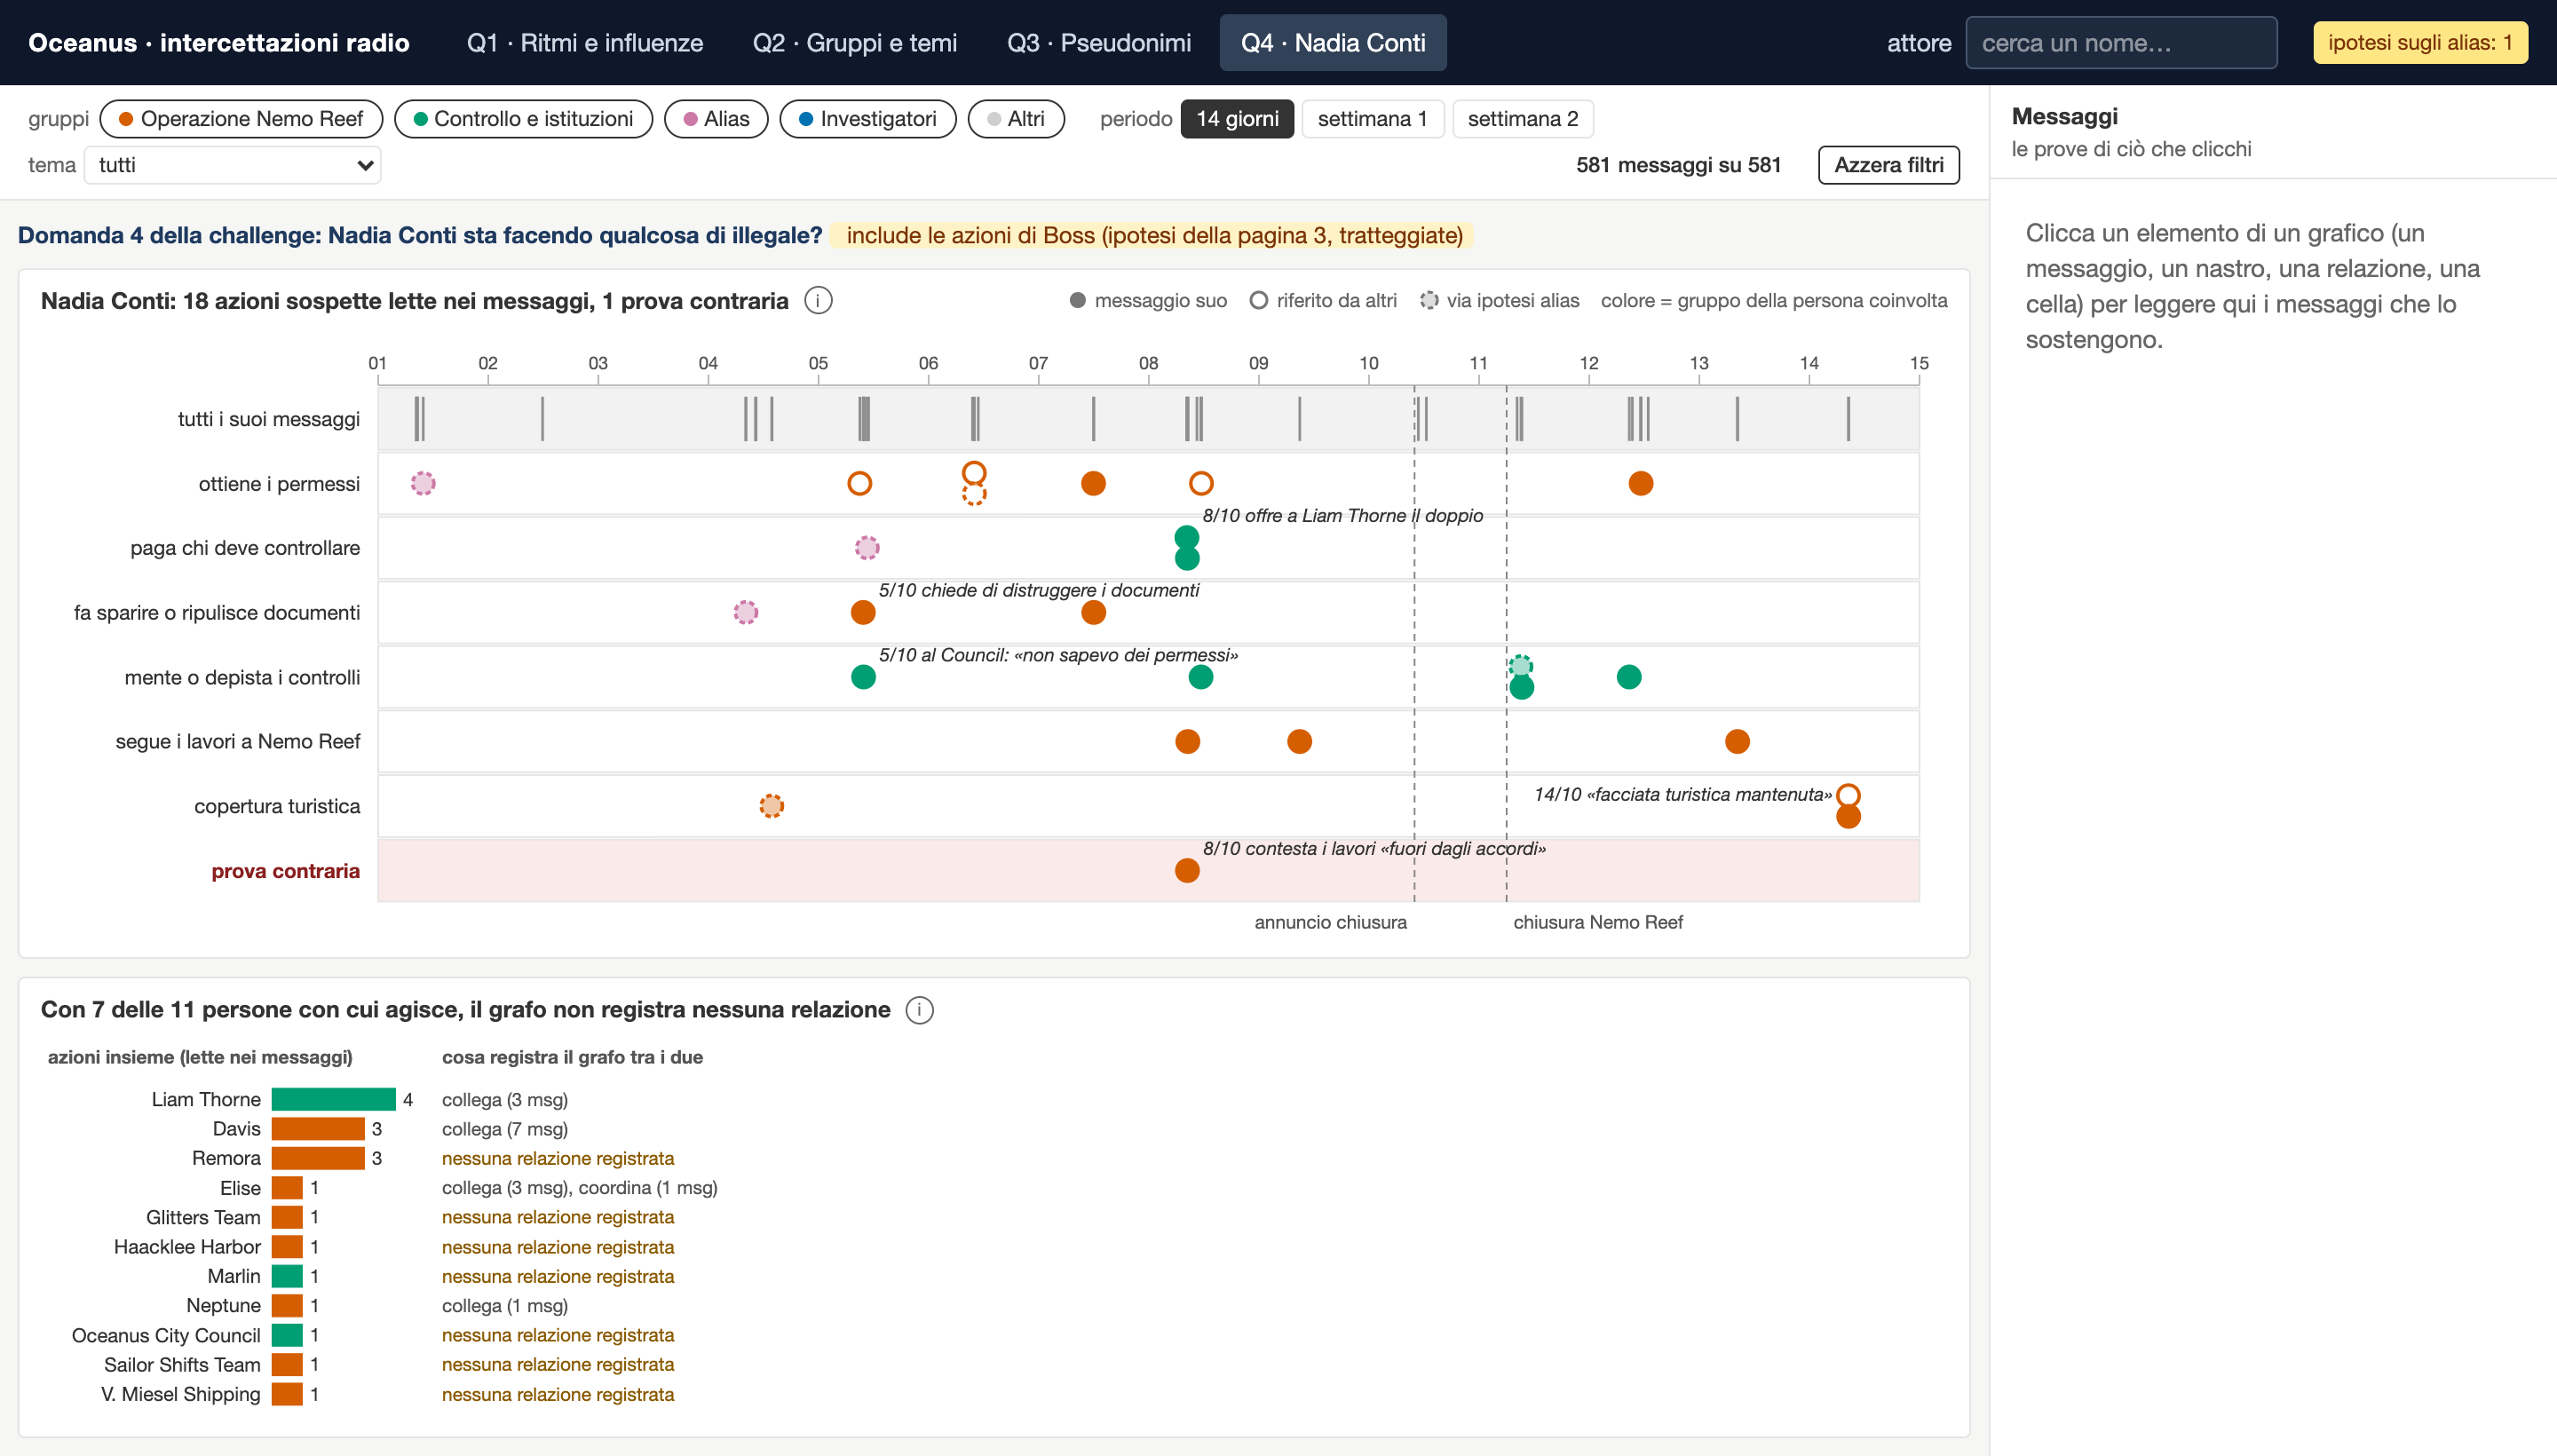
\includegraphics[width=\linewidth]{05_q3_ipotesi_boss_nadia.png}
\caption{Fourth page with the hypothesis ``Boss = Nadia Conti'' turned on: the actions of Boss appear dashed.}\label{fig:hypothesis}
\end{figure}

\subsection{Use case: Boss and Nadia Conti}
The journalist starts from the third page. The title of the ribbon view tells him that 74 of the 76 different
signatures are radio errors, so he should not treat them as pseudonyms. He chooses the alias Boss and the candidate
Nadia Conti: the title of the bar chart becomes ``Boss stops writing on the day Nadia Conti starts''. Clicking the bars
of 5 October he reads the last message of Boss (at 10:38) and the first ones of Nadia (from 9:45). Changing the
candidate, however, he sees that Elise, Rodriguez and Sam also write only after the last message of Boss, so this clue
alone is not enough. Choosing first Boss and then Nadia as the actor, on the fourth page he reads the messages in which they appear and
finds two pairs of almost simultaneous messages: on 6 October,
one minute apart, Glitters thanks Boss for the permits signed within hours by Commissioner Torres and Remora says that
it was Nadia who got Torres to sign; on 11 October Liam Thorne warns about the EcoVigil ROV first Boss and, 13 minutes
later, Nadia. At this point he turns on the hypothesis ``Boss = Nadia Conti'' and moves to the fourth page, where the
actions of Boss are added, dashed, to those of Nadia. Turning it off, he checks that the judgement on Nadia stays the
same without the hypothesis.

\subsection{Answers to the challenge questions}\label{sec:answers}
\paragraph{Question 1.} Messages are sent only between 8:00 and 15:00, but 83\% of the times cited in the texts fall
outside this band, mostly between 5:00 and 6:00 in the morning and between 21:00 and 22:00: the radio is used during the
day to organise activities that happen at dawn or in the evening. The day with most messages is 11 October (49), the
day of the closure of Nemo Reef. In the second week messages about \emph{closure of the area} (+55) and
\emph{equipment / works} (+51) increase, while those about the \emph{Sailor Shift event} ($-28$) and \emph{Nemo Reef}
($-26$) decrease; the Nemo Reef Operation group sends 25 more messages, the other groups fewer. As for influence, for
example, Remora is activated mostly by Mako (5 times) and in turn activates Rodriguez (9 times); Nadia Conti is
activated most often by Davis.

\paragraph{Question 2.} There are four groups: the Nemo Reef Operation (Nadia Conti, Davis, Elise, the vessels Mako,
Remora and Neptune, V.\ Miesel Shipping, the staff of Sailor Shift), Control and institutions (Oceanus City Council,
harbours, Green Guardians, patrol vessels, Liam Thorne), Aliases and Investigators. The aliases talk mostly among
themselves (75\% of their messages) and talk about money and payments much more than the other groups (49\% against at
most 8\%). Control and institutions talks mostly about Nemo Reef (64\%), the investigators about the environment (50\%)
and works (47\%), the Operation about permits (39\%) and works (36\%). Comparing the links of the messages with those of
the relationships shows ties that the intern's graph does not contain.

\paragraph{Question 3.}\label{sec:q3} The 74 signatures due to radio errors do not point to pseudonyms. The two
remaining cases are clues. In the first, the radio records Davis as the sender of a message signed Mako, and the graph
says that Davis operates the vessel Mako (13 supporting messages): Davis is therefore the captain speaking on behalf of
the vessel. In the second, on 13 October, the radio of The Middleman transmits a message signed The Accountant: they
could be the same person, but this rests on a single message and remains an open hypothesis. The best supported
hypothesis is that Nadia Conti is behind Boss, for the clues described in the use case: Boss stops writing on the day
she starts, they have contacts in common (Liam Thorne and V.\ Miesel Shipping) and two pairs of messages attribute the
same facts to both. It is not a proof, so in the application it remains a hypothesis that the analyst chooses to turn
on. For The Intern, The Lookout, Mrs.\ Money and The Middleman the messages are spread over the whole period and there
are not enough clues to link them to a person.

\paragraph{Question 4.} According to the messages, Nadia Conti is involved in illegal activities. On 5 October she asks
Haacklee Harbor to cancel the special corridor and to destroy the documents, and four minutes later she tells the
Council she knows nothing about the permits. On 7 October she asks Davis to create ``a clean paper trail''. On 8 October
she offers Liam Thorne double so that the Harbor Master ``cooperates'', and Liam confirms that he has moved the patrols.
Between 8 and 13 October she follows the equipment for the foundations, saying to stay ``under the radar'', and the
paperwork for permit \#CR-7844. On 14 October Remora tells her that the tourist facade is being maintained. In total
there are 18 actions, 14 in messages written or received by her and 4 reported by others. There is also one piece of
counter-evidence: on 8 October she complains to Neptune about foundation works ``outside the agreements''. It may be a
real disagreement about the works or a way of covering herself, but it does not change what emerges about permits and
payments. The result does not depend on the hypothesis about Boss, whose 6 actions appear only when the hypothesis is
on. Finally, for 7 of the 11 people she acts with the graph records no relationship at all: without reading the texts
these links would not be visible.

%---------------------------------------------------------------------
\section{Limitations and conclusions}
%---------------------------------------------------------------------
The application has some limitations:
\begin{itemize}
  \item topics are found with keywords, so there can be false positives or messages that are not recognised;
  \item I marked the suspicious actions by hand only for Nadia Conti and Boss; if another actor is chosen on the fourth
        page, their messages are shown but not their actions;
  \item the chart of who activates whom counts how many times an actor writes within 15 minutes after receiving a
        message: it shows who comes first in time, but it does not prove that one gives orders to the other;
  \item for pseudonyms no computed clue is enough on its own, and the hypotheses remain a choice of the analyst;
  \item the groups depend on the algorithm used (another method could change them slightly), and I chose their names myself;
  \item the correction of the senders assumes that the signature in the text is true;
  \item the interface is designed for a screen of at least 1440$\times$820 pixels.
\end{itemize}

In conclusion, the application allows answering the four questions starting from the rhythms of the communications,
going through the groups and the pseudonyms, up to the case of Nadia Conti. The most important point that emerged from
the work is the check of the senders: most of the ``suspicious'' signatures were radio errors, and correcting them
changes the results of every page. As future work, the coding of actions could be extended to the other actors,
hypotheses could be allowed between two aliases (such as The Middleman and The Accountant), and keywords could be
replaced by a topic classification model.

\end{document}
